\documentclass{beamer}
\beamertemplatenavigationsymbolsempty
% Theme selection
\usetheme{Madrid}
\usecolortheme{default} % You can change this to albatross, beaver, beetle, crane, dolphin, dove, fly, lily, orchid, rose, seagull, seahorse, whale, wolverine

% Document information
\title[Galaxy Classification]{Galaxy Morphology and Rotational Symmetry}
\subtitle{Classification on astroNN Galaxy10 SDSS dataset}
\author[unipr]{Leonardo Ongari \\ \vspace{0.3cm} \small \textit{Università degli Studi di Parma}}
\date[\today]{\today}

\begin{document}

% Title slide
\begin{frame}
    \titlepage
\end{frame}

% Table of contents
\begin{frame}{Outline}
    \tableofcontents
\end{frame}

\section{Introduction}
\begin{frame}{Introduction}
    \begin{itemize}
    \setlength\itemsep{2em}
        \item The dataset used is the original Galaxy10 SDSS file 
          containing 21,785 RGB images of size 69×69 pixels and corresponding labels
        \item The purpose of the project is to use supervised learning techniques 
          to solve the classification task
        \item Different approaches will be explored:
          \begin{itemize}
            \item Galaxy10CNN model
            \item Raw Learning (no augmentation)
            \item Data augmentation
          \end{itemize}
    \end{itemize}
\end{frame}

\section{Data Exploration and Visualization}
\begin{frame}{Problem Statement}
    \begin{figure}
      \centering
      \includegraphics[width=1\textwidth]{../plots/galaxies.pdf}
    \end{figure}
    \centering
    Example of 10 galaxies from the dataset
\end{frame}

\begin{frame}{Problem Statement}
    \begin{figure}
      \centering
      \includegraphics[width=0.6\textwidth]{../plots/balance.png}
    \end{figure}
    \centering
    The dataset is strongly unbalanced
\end{frame}

\begin{frame}{PCA}
    \begin{figure}
      \centering
      \includegraphics[width=0.7\textwidth]{../plots/pca.pdf}
    \end{figure}
    \centering
    Principle Component Analysis on the dataset
\end{frame}

\begin{frame}{LDA}
    \begin{figure}
      \centering
      \includegraphics[width=0.7\textwidth]{../plots/lda.pdf}
    \end{figure}
    \centering
    Linear Discriminant Analysis on train set
\end{frame}

\begin{frame}{LDA}
    \begin{figure}
      \centering
      \includegraphics[width=0.7\textwidth]{../plots/lda-test.pdf}
    \end{figure}
    \centering
    Linear Discriminant Analysis on test set (overfitting)
\end{frame}

\begin{frame}{Other Visualization Techniques}
    Other unsupervised methods were used to visualize data, including:
    \vspace{2em}

    \begin{itemize}
        \setlength\itemsep{2em}
        \item \textbf{UMAP} (Uniform Manifold Approximation and Projection)
        \item \textbf{t-SNE} (t-Student Stochastic Neighbor Embedding)
    \end{itemize}
    
\end{frame}

\section{Methodology}
\begin{frame}{Standard Approach}
    \begin{enumerate}
        \item \textbf{Phase 1:} Import dataset (manually or with galaxy10 SDSS loader)
        \item \textbf{Phase 2:} Preprocess data (grayscale, gaussian filter)
        \item \textbf{Phase 3:} Train and test the model 
    \end{enumerate}
    % 2 columns grid with images
    \begin{columns}
        \column{0.5\textwidth}
        \begin{figure}
          \centering
          
\includegraphics[width=0.8\textwidth]{../plots/gray.png}
          \caption{Grayscale data}
        \end{figure}
        
        \column{0.5\textwidth}
        \begin{figure}
          \centering
          \includegraphics[width=0.8\textwidth]{../plots/gauss.png}
          \caption{Gaussian filtered data}
        \end{figure}
    \end{columns}

\end{frame}

\begin{frame}{Galaxy10CNN}
    \begin{itemize}
        \item Inspired by Jupyter Notebook intro provided by astroNN
        \item Built-in simple 4 layered convolutional neural network 
            with 2 conv. layers and 2 dense layers
    \begin{figure}
      \centering
      \includegraphics[width=0.5\textwidth]{../plots/galaxy10CNN.png}
    \end{figure}
    \end{itemize}
\end{frame}

\begin{frame}{User Defined CNN - Raw Data}
    \begin{itemize}
        \item 3 convolutional blocks with increasing depth (8, 32, 64 filters), 
            each followed by MaxPooling 
        \item Each block targets deeper features of the images
        \item This model works on ``raw'' data without rotation or flips
    \end{itemize}
    \begin{columns}
        \column{0.5\textwidth}
        \begin{figure}
          \centering
          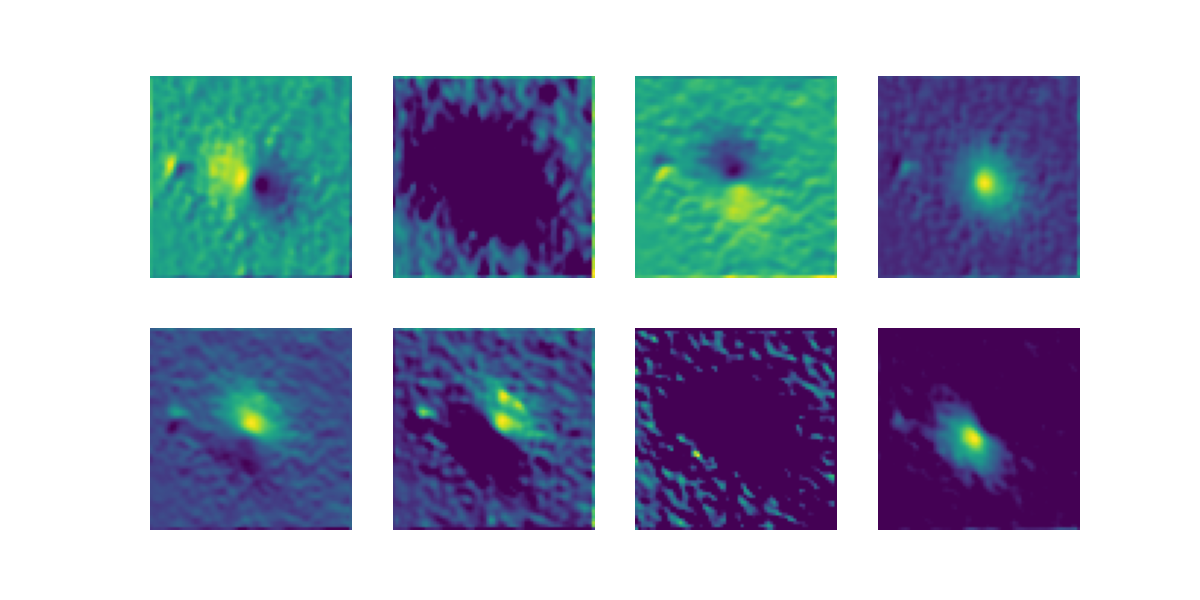
\includegraphics[width=\textwidth]{../learning_results/1LayerFM_no_smooth.png}
          \caption{First layer feature maps}
        \end{figure}
        
        \column{0.5\textwidth}
        \begin{figure}
          \centering
          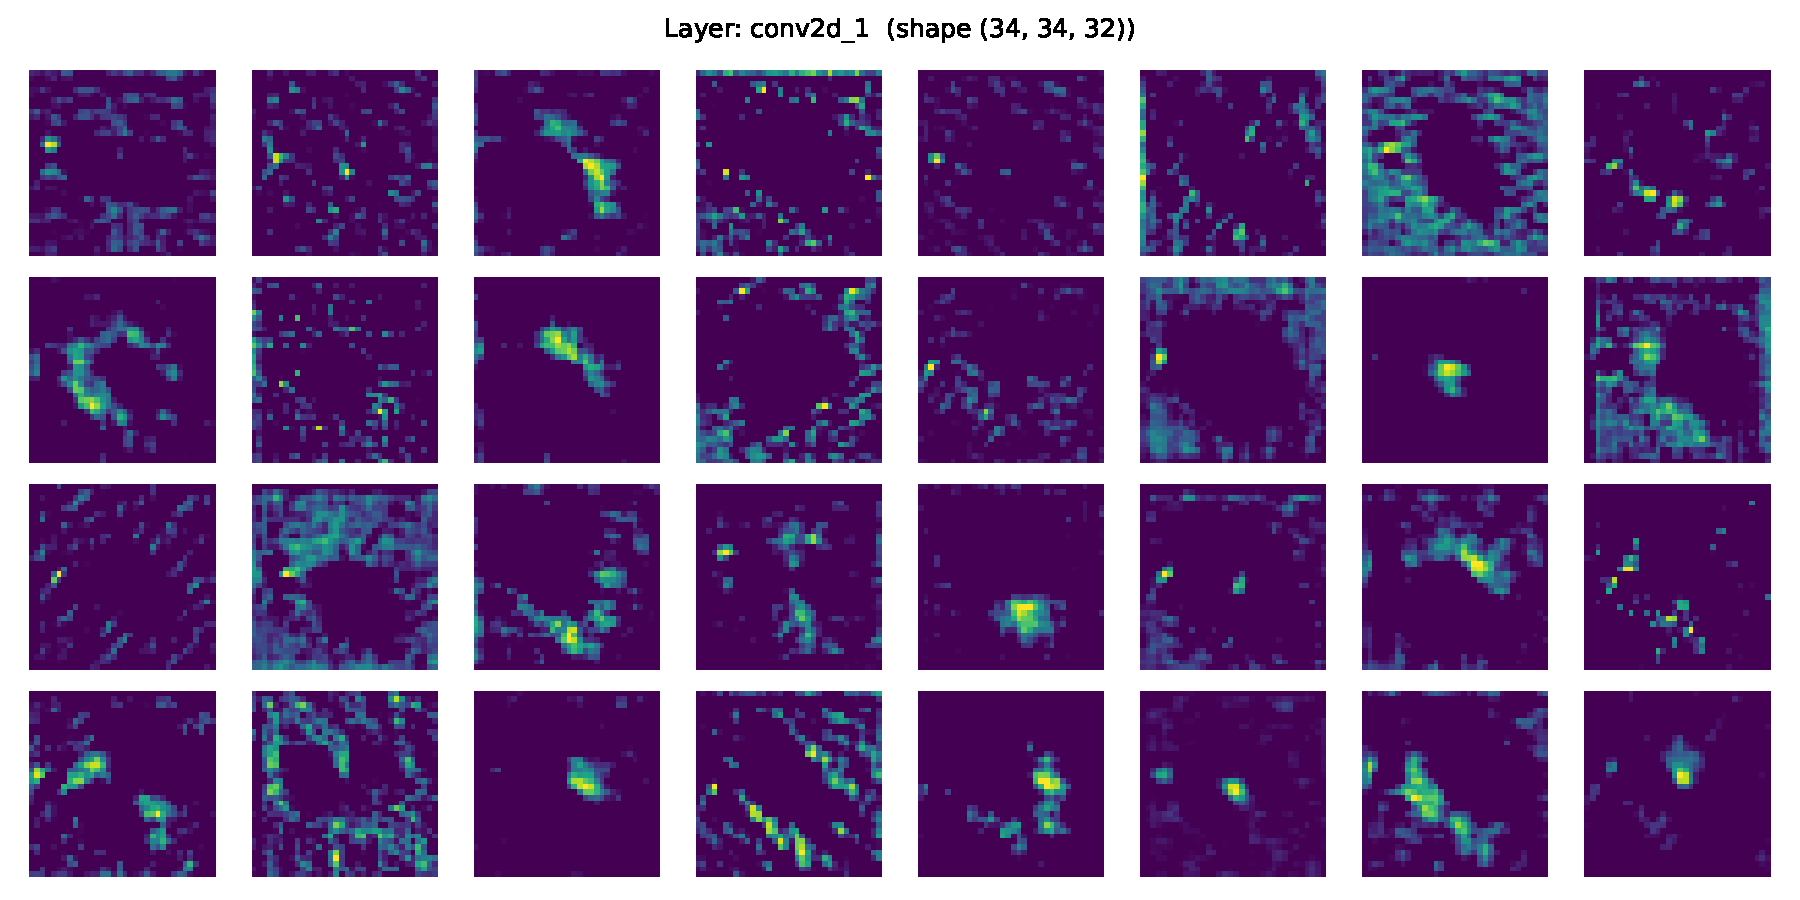
\includegraphics[width=\textwidth]{../learning_results/2LayerFM_no_smooth.pdf}
          \caption{Second layer feature maps}
        \end{figure}
    \end{columns}
\end{frame}

\begin{frame}{User Defined CNN - Data Augmentation}
    \begin{itemize}
    \setlength\itemsep{2em}
        \item Same format as the previous model, but with data augmentation applied
        \item Augmentation is done on the training set for each epoch and it includes:
        \begin{itemize}
            \item random flips (horizontally and vertically)
            \item random rotations (from -180 to 180 degrees)
        \end{itemize}
    \end{itemize}
\end{frame}

\section{Results}
\begin{frame}{Error on Training Set}
    \begin{itemize}
        \item 
    \end{itemize}
    \vspace{0.5cm}
    
    % Example of a simple table
    \begin{table}[]
        \centering
        \begin{tabular}{|l|c|r|}
            \hline
            \textbf{Phase} & \textbf{Status} & \textbf{Timeline} \\ \hline
            Phase 1 & \textcolor{green}{Completed} & Q1 2026 \\ \hline
            Phase 2 & \textcolor{blue}{In Progress} & Q2-Q3 2026 \\ \hline
            Phase 3 & \textcolor{gray}{Planned} & Q4 2026 \\ \hline
        \end{tabular}
        \caption{Current Project Timeline}
    \end{table}
\end{frame}

\section{Challenges \& Risks}
\begin{frame}{Challenges \& Risks}
    \begin{columns}
        \column{0.5\textwidth}
        \textbf{Identified Risks:}
        \begin{itemize}
            \item Resource constraints
            \item Technical dependencies
            \item Tight deadlines
        \end{itemize}
        
        \column{0.5\textwidth}
        \textbf{Mitigation Strategies:}
        \begin{itemize}
            \item Agile management
            \item Fallback plans
            \item Regular stakeholder check-ins
        \end{itemize}
    \end{columns}
\end{frame}

\section{Conclusion}
\begin{frame}{Conclusion \& Future Work}
    \begin{itemize}
        \item Summarize the main takeaways.
        \item Discuss the next steps or future enhancements.
        \item Acknowledge team members, advisors, or sponsors.
    \end{itemize}
\end{frame}

% Q&A Slide
\begin{frame}
    \centering \Huge
    \emph{Thank You!} \\
    \vspace{1cm}
    \Large Any Questions?
\end{frame}

\end{document}
